\XeTeXgenerateactualtext=1
\documentclass[fontset=none]{ctexbeamer}
% \documentclass[aspectratio=169]{ctexbeamer}

\usepackage{array,bookmark,ccicons,fontawesome,hologo,listings,ragged2e,siunitx,unicode-math}

\makeatletter

\@namedef{ver@beamerfontthememetropolis.sty}{9999/99/99}

% Beamer theme
\usetheme{Xiaoshan}
\usefonttheme{serif}
\usefonttheme{professionalfonts}

% Beamer settings
% \metroset{sectionpage=simple}
\metroset{progressbar=none}
\setbeamerfont{title}{size=\huge, series=\bfseries}
\setbeamerfont*{subtitle}{size=\large, shape=\itshape}
\setbeamerfont{section title}{size=\Large, series=\bfseries}
\setbeamerfont{frametitle}{size=\large, series=\bfseries}
\setbeamerfont{caption}{size=\footnotesize, series=\bfseries}
\setbeamerfont{footnote}{size=\tiny}
\setbeamerfont{alerted text}{series=\bfseries}
\addtobeamertemplate{institute}{\raggedleft}{}
\setbeamertemplate{title}{%
  \raggedleft
  \linespread{1.0}%
  \inserttitle
  \hspace*{1.2cm}\par
  \vspace*{0.5em}}
\setbeamertemplate{subtitle}{%
  \raggedleft
  \insertsubtitle
  \hspace*{1.2cm}\par
  \vspace*{0.5em}}
\setbeamertemplate{title page}{
  \begin{minipage}[b]{\textwidth}
    \mbox{}\vfill
    \usebeamertemplate*{title}
    \usebeamertemplate*{subtitle}
    \usebeamertemplate*{title separator}
    \usebeamertemplate*{author}
    \usebeamertemplate*{date}
    \usebeamertemplate*{institute}
    \vfill
  \end{minipage}}
\setbeamertemplate{frame numbering}{\zhnumber[style=Financial]{\insertframenumber}}
\setbeamertemplate{itemize/enumerate subbody begin}{\footnotesize}
\setbeamertemplate{caption}{\parbox{\textwidth}{\centering\insertcaption}\par}
\setbeamertemplate{bibliography item}[text]

% Colors
\colorlet{keyword}{松花绿}
\colorlet{comment}{漆黑!50}
\colorlet{texcs}{酡红}
\colorlet{emph1}{靛蓝}
\colorlet{emph2}{乌金}
\colorlet{inline}{玄色}

% Fonts
\setmainfont{Libertinus Serif}[Scale=1.1, BoldFont=* Bold]
\setsansfont{Roboto}
\setmonofont{Iosevka}
\setmathfont{Libertinus Math}
\setCJKmainfont{Source Han Serif SC}[%
  UprightFont=* SemiBold, BoldFont=* Heavy, ItalicFont=* SemiBold, RawFeature=+fwid]
\setCJKmonofont{Sarasa Mono SC}

% PDF bookmark
\apptocmd{\beamer@@frametitle}{%
  \only<1>{\expandafter\ifnum\insertcontinuationcount<2\relax
    \bookmark[page=\the\c@page,level=4]{#1}\fi}}{}{}

% Code listings
\lstdefinestyle{style@latex}{
  language     = [latex]TeX,
  alsoletter   = {*},
  basewidth    = 0.54em,
  basicstyle   = \small\ttfamily,
  keywordstyle = \bfseries\color{keyword},
  commentstyle = \itshape\color{comment},
  texcsstyle   = *\color{texcs},
  emphstyle    = [1]\itshape\color{emph1},
  emphstyle    = [2]\color{emph2}
}
\lstdefinestyle{style@inline}{
  basicstyle   = \ttfamily\color{inline},
  keepspaces   = true
}
\lstnewenvironment{texcode}[1][]{\lstset{
  style        = style@latex,
  gobble       = 2,
  morekeywords = {\documentclass,\usepackage,\begin,\end},#1}}{}
\lstMakeShortInline[style=style@inline]|

% Hack
% Use small caps for LaTeX symbol
\DeclareRobustCommand{\LaTeX}{%
  L\kern-.3em%
  \raisebox{.2em}{\textsc{a}}\kern-.14em%
  \TeX}
% Compatibility with unicode-math
\DeclareRobustCommand{\LaTeXe}{%
  \LaTeX\kern.15em2%
  \hbox{%
    \if b\expandafter\@car\f@series\@nil
      $_{\textstyle\symbf{\varepsilon}}$%
    \else
      $_{\textstyle\varepsilon}$%
    \fi}}
% PoZheHao, see https://github.com/CTeX-org/ctex-kit/issues/382
\ExplSyntaxOn
\xeCJK_new_class:n { PoZheHao }
\__xeCJK_save_CJK_class:n { PoZheHao }
\xeCJK_declare_char_class:nn { PoZheHao } { "2014 }
\seq_map_inline:Nn \g__xeCJK_class_seq
  {
    \str_if_eq:nnF {#1} { PoZheHao }
      {
        \xeCJK_copy_inter_class_toks:nnnn { PoZheHao } {#1} { FullRight } {#1}
        \xeCJK_copy_inter_class_toks:nnnn {#1} { PoZheHao } {#1} { FullRight }
      }
  }
\ExplSyntaxOff

% Macros
\newcommand\link[1]{\href{#1}{\faLink}}
\newcommand\CASE[1]{{\addfontfeatures{Letters=Uppercase}#1}}
\newcommand\zhparen[1]{(\raisebox{0.1ex}{#1})}
\newcommand\enparen[1]{\CASE{(}#1\CASE{)}}
\newcommand\pkg[1]{\texttt{#1}}
\newcommand\usv[1]{\texttt{U+#1}}
\newcommand\kbd[1]{{\fontspec{Libertinus Keyboard}#1}}
\newcommand\kbdWin{{\fontspec{Libertinus Keyboard}\symbol{"E168}}}
\newcommand\kbdAlt{{\fontspec{Libertinus Keyboard}\symbol{"E171}}}
\newcommand\kbdCtrl{{\fontspec{Libertinus Keyboard}\symbol{"E173}}}
\newcommand\kbdShift{{\fontspec{Libertinus Keyboard}\symbol{"E174}}}
\newcommand\kbdIns{{\fontspec{Libertinus Keyboard}\symbol{"E18B}}}
\DeclareRobustCommand{\nonumberfootnote}[1]{
  \let\thefootnote\relax
  \footnotetext{#1}}

\newcommand\XeTeX{\hologo{XeTeX}}
\newcommand\pdfTeX{\hologo{pdfTeX}}
\newcommand\LuaTeX{\hologo{LuaTeX}}
\newcommand\XeLaTeX{\hologo{Xe}\kern-.13em\LaTeX{}}
\newcommand\pdfLaTeX{pdf\LaTeX{}}
\newcommand\LuaLaTeX{Lua\LaTeX{}}
\newcommand\BibTeX{\hologo{BibTeX}}

\makeatother

% Information
\title{现代 \LaTeX{} 入门讲座}
\subtitle{Modern \LaTeX{} in a Nutshell}
\author{曾祥东}
\institute{复旦大学\quad 物理系}
\date{2018 年 12 月}

\begin{document}

\maketitle

%\begin{frame}[standout]
  \large\xkcd
  ``Your paper makes no goddamn sense, \\
  but it's the most beautiful thing \\
  \XeTeXglyph\XeTeXglyphindex"I_hyphen_p_r_o_n_o_u_n"\relax\
  have ever laid eyes on.''

  \small
  \hfill From r/ProgrammerHumor
  \href{https://www.reddit.com/r/ProgrammerHumor/comments/2jf7yl}{\faRedditAlien}
\end{frame}

\section{介绍}

\begin{frame}{历史回眸}
\begin{columns}
\begin{column}{0.45\textwidth}
  \begin{figure}
    \centering
    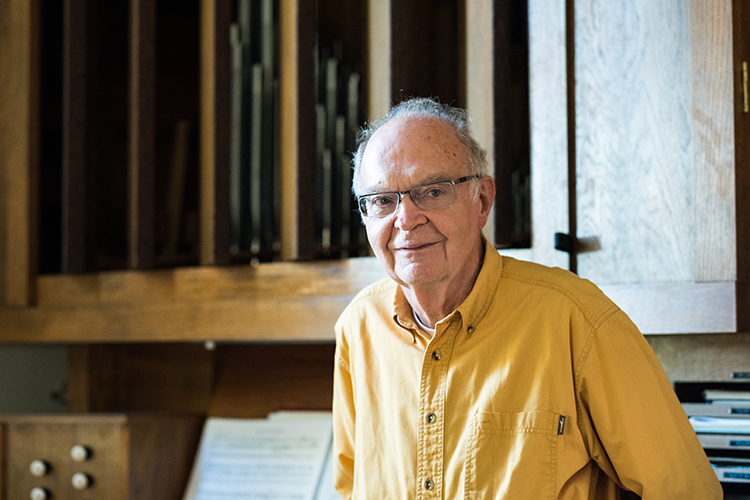
\includegraphics[height=3.2cm]{figures/Knuth-vivian20181019E.jpg}
    \caption{高德纳(Donald~E. Knuth) \\ \TeX}
  \end{figure}
\end{column}
\begin{column}{0.45\textwidth}
  \begin{figure}
    \centering
    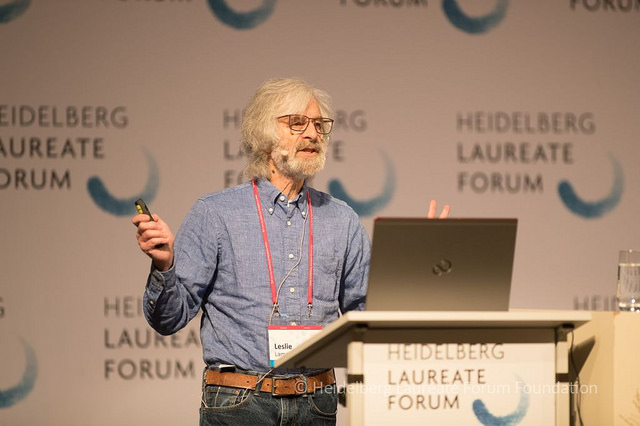
\includegraphics[height=3.2cm]{figures/lamport-2018.jpg}
    \caption{Leslie Lamport \\ \LaTeX}
  \end{figure}
\end{column}
\end{columns}
\nonumberfootnote{图片来源:
  \link{https://www-cs-faculty.stanford.edu/~knuth/graphics.html}
  \link{https://aperiodical.com/2018/09/hlf-blogs-leslie-lamport-thinks-your-code-is-bad}}
\end{frame}

\begin{frame}{\LaTeX{} 是什么?}
\pause
\begin{itemize}
  \item 打公式方便?
  \item 写论文神器?
  \item 排版语言 + 标记语言 + 宏语言?
\end{itemize}
\end{frame}

\begin{frame}[fragile]
\frametitle{\LaTeX{} 是什么?\mbox{}——\mbox{}What you \emph{think} is what you get!}
\begin{columns}
\begin{column}{0.48\textwidth}
  \begin{texcode}[basicstyle=\tiny\ttfamily, moretexcs={\maketitle},
    emph={[1]equation,itemize,document},emph={[2]article,amsmath,graphicx}]
  \documentclass{article}
  \usepackage{amsmath,graphicx}
  \title{Normal distribution}
  \author{Wikipedia, the free encyclopedia}

  \begin{document}
  \maketitle
  \section{Introduction}
  % 省略一些内容……
  The probability density of the normal
  distribution is
  \begin{equation}
    f(x|\mu, \sigma)
    = \frac{1}{\sqrt{2\pi\sigma^2}}
      e^{-\frac{(x-\mu)^2}{2\sigma^2}}
  \end{equation}
  where
  \begin{itemize}
    \item $\mu$ is the mean of the distribution
    \item $\sigma$ is the standard deviation
  \end{itemize}
  \end{document}
  \end{texcode}
\end{column}
\pause
\begin{column}{0.48\textwidth}
  \begin{figure}
    \centering
    \vspace{-0.8cm}
    \includegraphics[width=\textwidth]{example/normal-dist.pdf}
  \end{figure}
\end{column}
\end{columns}
\nonumberfootnote{来源:Wikipedia \link{https://en.wikipedia.org/wiki/Normal_distribution}}
\end{frame}

\begin{frame}{基本原则}
\begin{itemize}
  \item<+-> 排版 \textit{vs} 文字处理
    \begin{itemize}
      \item 《别把 \LaTeX{} 当 Word 用》
    \end{itemize}
  \item<+-> 遵循业\zhparen{xué}界\zhparen{xiào}规范
    \begin{itemize}
      \item 《管教务处 \textit{or} 研究生院 \textit{or} 物理系叫爸爸》
    \end{itemize}
  \item<+-> 追求良好的阅读体验\zhparen{readability}
  \item<+-> 内容与格式分离
  \item<+-> \alert{内容永远比格式重要!}
\end{itemize}
\end{frame}

%\section{安装}

\begin{frame}{选择发行版}
\begin{itemize}
  \item \TeX{} 发行版\zhparen{distribution}

    \begin{itemize}
      \item 引擎、宏包、字体、文档的综合体
      \item 类比 Visual Studio
      \item \TeX{} Live、Mac\TeX{}、W32\TeX{}、MiK\TeX{} 等
    \end{itemize} \pause

  \item \TeX{} Live \link{https://www.tug.org/texlive}

    \begin{itemize}
      \item 官方维护,首选,跨平台
      \item Mac\TeX{} ≈ macOS 下的 \TeX{} Live
      \item 缺点:体积大\zhparen{3GB+}、每年需要重装(2019 版将于月底发布)
    \end{itemize}

  \item MiK\TeX{} \link{https://miktex.org}

    \begin{itemize}
      \item 由 Christian Schenk 维护(是个狠人)
      \item 宏包随用随装
      \item 缺点:曾经只有 Windows 版本、网络问题
    \end{itemize} \pause

  \item \alert{不要安装 \CTeX{} 套装!}

    \begin{itemize}
      \item \alert{存在严重 bug,并且完全过时}
    \end{itemize}
\end{itemize}
\end{frame}

\begin{frame}{下载}
\begin{itemize}
  \item 选择国内 CTAN 镜像

    \begin{itemize}
      \item 清华大学开源软件镜像站 \link{https://mirrors.tuna.tsinghua.edu.cn}
      \item 上海交通大学软件源镜像服务 \link{https://mirrors.sjtug.sjtu.edu.cn}
      \item 中国科学技术大学开源软件镜像 \link{https://mirrors.ustc.edu.cn} \pause
      \item 复旦大学……
    \end{itemize} \pause

  \item 建议使用 ISO 镜像离线安装
  \item 在线安装要求网络稳定
\end{itemize}
\end{frame}

\begin{frame}{安装流程}
\begin{itemize}
  \item 新手建议安装完整版 \TeX{} Live 或 Mac\TeX{}

    \begin{itemize}
      \item 一路点击「下一步」
      \item 保持耐心,做好重装的打算
    \end{itemize}

  \item<+-> Linux specials

    \begin{itemize}
      \item 软件源更新较慢,可以考虑 Vanilla \TeX{} Live
      \item GUI 安装界面需要 \pkg{perl-tk} 等
      \item 环境变量、\pkg{fontconfig}、dummy package 配置
    \end{itemize}
\end{itemize}
\end{frame}

\begin{frame}[fragile]
\frametitle{神圣的战争——选择编辑器}
\begin{itemize}
  \item<+-> 专用型

    \begin{itemize}
      \item TeXworks:\TeX{} Live 自带 \faWindows{} \faApple{} \faLinux{}
      \item TeXstudio:功能丰富,对新手友好 \faWindows{} \faApple{} \faLinux{}
      \item TeXShop:Mac\TeX{} 自带 \faApple{}
      \item WinEdt:功能丰富,收费 \faWindows{}
    \end{itemize}

  \item<+-> 通用型

    \begin{itemize}
      \item Visual Studio Code:利益相关(逃
      \item Atom:卡
      \item Sublime Text:收费
      \item Vim:|q|、|q!|、|wq|、|wq!|
    \end{itemize}

  \item<+-> 在线服务

    \begin{itemize}
      \item \href{https://www.sharelatex.com}{\textcolor{酡红}{ShareLaTeX}} 和
            \href{https://www.overleaf.com}{\textcolor{松花绿}{Overleaf}}(现已合并)
    \end{itemize}

  \item<+-> 编辑器对比:\link{https://tex.stackexchange.com/q/339}
                        \link{https://en.wikipedia.org/wiki/Comparison_of_TeX_editors}
                        \link{https://www.zhihu.com/question/19954023}
\end{itemize}
\end{frame}

%\section{开始之前……}

\begin{frame}[fragile]
\frametitle{命令行基础}
\begin{itemize}
  \item 打开终端

    \begin{itemize}
      \item \faWindows{}:右键开始菜单、空白处 \kbd{Shift} + 右键、\kbd{Windows} + \kbd{R} \& |cmd|
      \item \faLinux{}:\kbd{Ctrl} + \kbd{Alt} + \kbd{T}
      \item \faApple{}:\kbd{⌘} + \kbd{Space} 搜索 Terminal、可在 Finder 中添加服务
    \end{itemize}

  \item 基本命令:

    \begin{itemize}
      \item |cd|、|ls/dir|、|rm/del|、|clear/cls|
      \item 选项:|-h|、|--help|、|/?|
    \end{itemize}

  \item 其他:

    \begin{itemize}
      \item 复制粘贴:\kbd{Ctrl}/\kbd{Shift} + \kbd{Ins}、\kbd{Ctrl}/\kbd{⌘} + \kbd{C}/\kbd{V}、
      \item 路径连接符:斜线(|/|)或反斜线(|\|)
      \item 换行符:LF(|\n|)或 CRLF(|\r\n|)
      \item 结束进程:\kbd{Ctrl} + \kbd{C}
    \end{itemize} \pause

  \item \alert{尽量不要用中文;避免空格、特殊符号}
\end{itemize}
\end{frame}

\begin{frame}{编码}
关于 \LaTeX{} 源文件的编码,我们给出如下结论:\pause
\begin{alertblock}{编码定理}
  一般地,在任何场合使用(不带 BOM)的 \alert{UTF\CASE{-}8} 编码均是最优选择.
\end{alertblock} \pause
此定理的证明留做习题.
\end{frame}

%\section{填写内容}

\begin{frame}[fragile]
\frametitle{Hello world!}
\begin{texcode}[emph={[1]document}, emph={[2]article}]
  % 用 pdfLaTeX、XeLaTeX 或 LuaLaTeX 编译
  \documentclass{article}
  \begin{document}
  Hello world!
  \end{document}
\end{texcode}

\begin{texcode}[emph={[1]document}, emph={[2]ctexart}]
  % 用 XeLaTeX 或 LuaLaTeX 编译
  \documentclass{ctexart}
  \begin{document}
  你好,世界!
  \end{document}
  \end{texcode}
\end{frame}

\begin{frame}{引擎与格式}
\begin{itemize}
  \item \textbf{引擎}:\TeX{} 的实现
    \begin{itemize}
      \item \pdfTeX{}:直接生成 PDF,支持 micro-typography
      \item \XeTeX{}:支持 Unicode、OpenType 与复杂文本排版
      \item \LuaTeX{}:支持 Unicode,内联 Lua,支持 OpenType
      \item Ap\TeX{}:底层 CJK 支持,内联 Ruby,Color Emoji(手动斜眼笑)
    \end{itemize}
  \item \textbf{格式}:\TeX{} 的语言扩展(命令封装)
    \begin{itemize}
      \item plain \TeX{}:Knuth 同志专用
      \item \LaTeX{}:排版科技类文章的事实\zhparen{\textit{de facto}}标准
      \item Con\TeX t:基于 \LuaTeX{} 实现,优雅、易用(吗?)
    \end{itemize}
  \item \textbf{程序}:引擎 + dump 之后的格式代码
    \begin{itemize}
      \item \alert{英文文章:\exe{pdflatex}、\exe{xelatex} 或 \exe{lualatex}}
      \item \alert{中文文章:\exe{xelatex} 或 \exe{lualatex}}
    \end{itemize}
\end{itemize}
\end{frame}

\begin{frame}[fragile]
\frametitle{语法}
\begin{itemize}
  \item 注释以 |%| 开头,忽略其后所有内容
  \item 命令以 |\| 开头,区分大小写
    \begin{itemize}
      \item |\foo{arg}|:必选参数放在 |{...}| 中
      \item |\foo[bar]{arg}|:可选参数放在 |[...]|
    \end{itemize}
  \item 环境
    \begin{texcode}[gobble=4, basicstyle=\footnotesize\ttfamily, emph={[1]env}]
      \begin{env}
        ...
      \end{env}
    \end{texcode}
  \item 特殊符号需要转义:|\%|、|\$|、|\&| 等
  \item 连续多个空格 = 单个空格 = 单个换行符
  \item \TeX{}/\LaTeX{} 的语法可以修改
\end{itemize}
\end{frame}

\begin{frame}[fragile]
\frametitle{文件结构}
\begin{texcode}[basicstyle=\scriptsize\ttfamily, moretexcs={\keyword,\boldsymbol},
  emph={[1]document}, emph={[2]article,amsmath}]
  % 用 UTF-8 编码,命名为 xxx.tex
  \documentclass{article}                     % 指明文档类型:文章
  % 导言区:设置文档样式
  \usepackage{amsmath}                        % 调用宏包,实现各种功能
  \newcommand\keyword[1]{\textbf{#1}}         % 自定义命令

  \begin{document}
  % 正文:套用格式
  In quantum mechanics, the \keyword{Schr\"odinger equation} is a
  mathematical equation that describes the changes over time of a
  physical system in which quantum effects, such as \keyword{wave--%
  particle duality}, are significant.

  % 上面的空行表示分段
  In classical mechanics, Newton's second law
  ($\boldsymbol{F}=m\boldsymbol{a}$) is used to make a \ldots{}

  Time-dependent Schrödinger equation can be written as  % ö 也能直接用
  \[ i\hbar \frac{d}{dt} |\Psi(t)\rangle = \hat{H} |\Psi(t)\rangle. \]
  \end{document}
\end{texcode}
\vspace{-0.6cm}
\end{frame}

\begin{frame}{Schrödinger equation}
In quantum mechanics, the \textbf{Schr\"odinger equation} is a
mathematical equation that describes the changes over time of a
physical system in which quantum effects, such as \textbf{wave--%
particle duality}, are significant.

In classical mechanics, Newton's second law
($\boldsymbol{F}=m\boldsymbol{a}$) is used to make a \ldots{}

Time-dependent Schrödinger equation can be written as
\[ i\hbar \frac{d}{dt} \vert\Psi(t)\rangle = \hat{H} \, \vert\Psi(t)\rangle. \]
\end{frame}

\begin{frame}[fragile]
\frametitle{谋篇布局}
\begin{itemize}
  \item 文档部件
    \begin{itemize}
      \item 标题:|\title|、|\author|、|\date| $\to$ |\maketitle|
      \item 摘要:|abstract| 环境
      \item 目录:|\tableofcontents|
      \item 章节:|\chapter|、|\section|、|\subsection| 等
      \item 文献:|\bibliography|
    \end{itemize}
  \item 文档划分
    \begin{itemize}
      \item 凤头猪肚豹尾:|\frontmatter|、|\mainmatter|、|\backmatter|
      \item 分文件编译:|\include|、|\input|
    \end{itemize}
\end{itemize}
\end{frame}

\begin{frame}[fragile]
\frametitle{文本标记}
\begin{itemize}
  \item 加粗:|{\bfseries ...}| 或 |\textbf{...}|
  \item 倾斜:|{\itshape ...}| 或 |\textit{...}|
  \item 字号:|\tiny|、|\small|、|\large|、|\Large| 等
  \item 换行:|\\|
  \item 缩进:|\indent|
  \item 居中:|\centering| 或 |center| 环境
\end{itemize}
\end{frame}

\begin{frame}[standout]
  \huge \textbf{请忘记上一页}
\end{frame}

\begin{frame}[fragile]
\frametitle{文本标记}
\begin{itemize}
  \item 为什么要有不同的标记?\mbox{}——表达不同的\alert{语义}
  \item |\textbf| 这样的命令是否表达语义?
  \item 再提一遍基本原则:\alert{内容与格式分离}
  \item 正确(或曰:合理)的做法
    \begin{itemize}
      \item 强调文字(意大利体):|\emph{...}|
      \item 摘要(居中,小字号,带有标题):|abstract| 环境
      \item 引用(左右边距较大):|quote| 或 |quotation| 环境
      \item 自定义新的命令、环境
    \end{itemize}
  \item 报告,我想偷懒!
\end{itemize}
\end{frame}

\begin{frame}{中文支持}
\begin{columns}
\begin{column}{0.65\textwidth}
  \begin{itemize}
    \item 中文有什么特殊?
      \begin{itemize}
        \item 汉字太多(87,887)
        \item 横排 + 直排、标点禁则、行间注 \link{https://www.w3.org/TR/clreq}
        \item {\CJKfontspec{Source Han Serif SemiBold}日本語(にほんご)}、
              {\fontspec{FreeSerif}[Script=Devanagari]देवनागरी}、
              {\fontspec{FreeSerif}[Script=Arabic]العَرَبِيَّة‎}
      \end{itemize}
    \item 已淘汰:
      \begin{itemize}
        \item CCT 系统、\pkg{CJK} 宏包(裸用)
        \item \CTeX{} 套装
      \end{itemize}
    \item 目前推荐手段:
      \begin{itemize}
        \item \alert{\CTeX{} 宏集}(此 \CTeX{} 非彼 \CTeX{})
        \item \exe{xelatex} 编译
      \end{itemize}
    \item 可以用,不推荐:
      \begin{itemize}
        \item \pkg{xeCJK} 宏包(裸用)
        \item \CTeX{} 宏集 + 其他引擎编译
      \end{itemize}
  \end{itemize}
\end{column}
\begin{column}{0.33\textwidth}
  \tiny
  \begin{tabular}{cc}
    
\includegraphics[width=1cm]{figures/leoliu.png}        &
    
\includegraphics[width=1cm]{figures/qinglee.jpg}       \\
    刘海洋 & 李清 \\[2ex]
    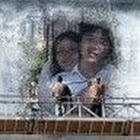
\includegraphics[width=1cm]{figures/wulingyun.jpg}     &
    
\includegraphics[width=1cm]{figures/jjgod.jpg}         \\
    吴凌云 & 江疆 \\[2ex]
    
\includegraphics[width=1cm]{figures/li-a-ling.jpg}     &
    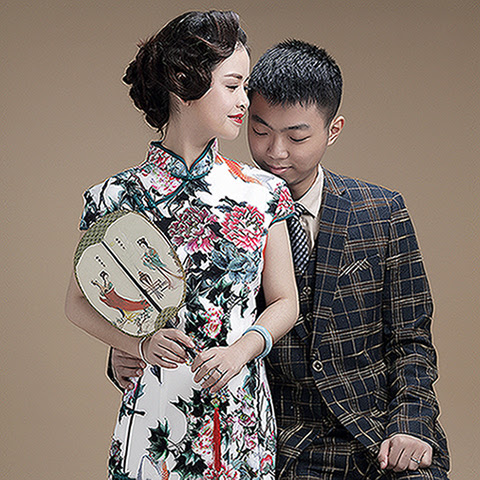
\includegraphics[width=1cm]{figures/liam-huang.jpg}    \\
    马起园 & 黄晨成 \\[2ex]
    
\includegraphics[width=1cm]{figures/louisstuart96.jpg} &
    
\includegraphics[width=1cm]{figures/zepinglee.jpg}     \\
    鲁尚文 & 李泽平
  \end{tabular}
\end{column}
\end{columns}
\let\thefootnote\relax
\footnotetext{图片来源:Github,知乎}
\end{frame}

\begin{frame}[fragile]
\frametitle{模板}
\begin{itemize}
  \item 是什么?
    \begin{itemize}
      \item 设计好的格式框架
      \item 专注于内容
      \item Word 中的样式:「学好 \LaTeX{} 可以更科学地使用 Word」
    \end{itemize}
  \item 有哪些?
    \begin{itemize}
      \item 期刊:REV\TeX{}、\pkg{elsarticle}、\pkg{IEEEtran}……
      \item 学位论文:\pkg{thuthesis}、\pkg{ustcthesis}、\alert{\pkg{fduthesis}}……
    \end{itemize}
  \item 怎么用?
    \begin{itemize}
      \item |\documentclass{...}|,配置参数,照常编写
      \item \alert{看文档,看文档,看文档}
    \end{itemize}
  \item 去哪里找?
    \begin{itemize}
      \item CTAN \link{https://ctan.org} 或 GitHub \href{https://github.com}{\faGithub}
      \item 期刊官网
      \item 「湿兄用 U 盘拷给你的模板一定是过时的」
    \end{itemize}
\end{itemize}
\end{frame}

%\section{公式}

\begin{frame}[fragile]
\frametitle{数学模式}
\begin{itemize}
  \item<+-> 一切数学公式都要在数学模式下输入

    \begin{itemize}
      \item 不受外界字体命令控制
      \item 数学模式中空格不起作用,尽管用
      \item \alert{不建议用 MathType 生成 \LaTeX{} 公式}
    \end{itemize}

  \item<+-> 行内\zhparen{inline}公式

    \begin{itemize}
      \item 用一对美元符号(公式值千金):|$...$|
      \item 示例:理想气体状态方程可以写为 $PV=nRT$, 其中 $P$、$V$ 和 $T$
        分别是压强、体积和绝对温度
    \end{itemize}

  \item<+-> 独显\zhparen{display}公式

    \begin{itemize}
      \item 无编号:用 |\[...\]| 或 |equation*| 环境
      \item 编号:用 |equation| 环境
      \item 多行:\pkg{amsmath} 宏包提供的 |gather|、|align|、|mutiline| 等环境
      \item \alert{不要用} |$$...$$| \alert{和} |eqnarray| \alert{环境}
    \end{itemize}
\end{itemize}
\end{frame}

\begin{frame}[fragile]
\frametitle{结构}
\begin{itemize}
  \item 上下标

    \begin{itemize}
      \item |^| 和 |_|
      \item 注意编组:|f^ab| 和 |f^{ab}|,|e^x^2|、|{e^x}^2| 和 |e^{x^2}|
      \item 张量:|R^a{}_b{}^{cd}| 或使用 \pkg{tensor} 宏包
      \item 配合积分、求和、极限使用:|\int|、|\sum|、|\limit|
    \end{itemize}

  \item 分式

    \begin{itemize}
      \item |\frac{〈分子〉}{〈分母〉}|
      \item 行内分式、小分式不好看:改用 |a/b|,或改用独显公式
      \item \alert{不推荐} |\dfrac|
    \end{itemize}

  \item 根式

    \begin{itemize}
      \item |\sqrt[〈次数〉]{〈内容〉}|
      \item 复杂情况改用分数指数:|{...}^{1/n}|
    \end{itemize}
\end{itemize}
\end{frame}

\begin{frame}[fragile]
\frametitle{括号与定界符}
\begin{itemize}
  \item<+-> 基本括号

    \begin{itemize}
      \item |(...)|、|[...]|、|\{...\}|、
      \item 绝对值、范数:\lstinline[style=style@inline]+|...|+ 或 |\vert...\vert|、|\Vert...\Vert|
      \item Dirac 符号:|\angle...\rangle|、\lstinline[style=style@inline]+|...\rangle+
    \end{itemize}

  \item<+-> 自动调节

    \begin{itemize}
      \item |\left(...\right)| 等
      \item 大型括号是拼出来的
    \end{itemize}

  \item<+-> 手动调节

    \begin{itemize}
      \item 只有 4 + 1 档:|\big|、|\Big|、|\bigg|、|\Bigg|
      \item 声明左中右:|\bigl|、|\bigm|、|\bigr| 等
    \end{itemize}
\end{itemize}
\end{frame}

\begin{frame}{符号与字体}
\begin{itemize}
  \item 符号不是 \LaTeX{} 画出来的,也不是天上掉下来的 \pause

    \begin{itemize}
      \item (几乎)所有的符号都由字体提供 \pause
      \item 分清「它是什么」和「它长什么样」(术语:character 和 glyph)
    \end{itemize} \pause

  \item 寻找符号

    \begin{itemize}
      \item S. Pakin. \emph{The Comprehensive \LaTeX{} Symbol List}
            \link{https://ctan.org/pkg/comprehensive}
      \item 手写识别(不全):Detexify \link{http://detexify.kirelabs.org}
    \end{itemize} \pause

  \item 数学字体

    \begin{itemize}
      \item 你们要的「Times New Roman」:\pkg{newtxmath} 宏包
      \item \alert{不要用 \pkg{times} 和 \pkg{mathptmx} 宏包}
      \item 加粗:使用 \pkg{bm} 宏包
    \end{itemize} \pause

  \item 新方案:\pkg{unicode-math}

    \begin{itemize}
      \item 彻底修改底层,不可以混用
    \end{itemize}
\end{itemize}
\end{frame}

\begin{frame}[fragile]
\frametitle{专业功能(一)}
\begin{itemize}
  \item 更高更妙的物理:\pkg{physics} 宏包

    \begin{itemize}
      \item 括号:|\qty()|、|\qty\big{...}|
      \item Dirac 符号:|\ket|、|\bra|、|\ev|
      \item 向量、导数、微分、矩阵……
    \end{itemize} \pause

  \item 国际单位:\pkg{siunitx} 宏包

    \begin{itemize}
      \item |$1.23 J mol^{-1} K^{-1}$|

        \begin{itemize}
          \item $1.23 J mol^{-1} K^{-1}$---No!
        \end{itemize}

      \item |\SI{1.23}{J.mol^{-1}.K^{-1}}|

        \begin{itemize}
          \item \SI{1.23}{J.mol^{-1}.K^{-1}}---Yes!
        \end{itemize} \pause

      \item 注 1:此宏包代码比 \LaTeX{} 内核还长 \pause
      \item 注 2:新定义并不会影响使用
            \link{https://en.wikipedia.org/wiki/2019_redefinition_of_SI_base_units}
    \end{itemize}
\end{itemize}
\end{frame}

\begin{frame}{专业功能(二)}
\begin{columns}
\begin{column}{0.65\textwidth}
  \begin{itemize}
    \item 花式图表

      \begin{itemize}
        \item Feynman 图:\pkg{tikz-feynman} 宏包%
              \zhparen{arXiv: 1601.05437 \link{https://arxiv.org/abs/1601.05437}}
        \item Feynman 斜线:\pkg{slashed} 宏包
        \item Wick 定理:\pkg{simplewick} 宏包、\pkg{simpler-wick} 宏包
        \item Young 表、Young 图:\pkg{ytableau} 宏包
        \item 电路图:\pkg{circuitikz} 宏包
        \item 拓扑量子场论:\pkg{tqft} 宏包
        \item ……
      \end{itemize}
  \end{itemize}
\end{column} \pause
\begin{column}{0.3\textwidth}
  \hspace{-0.15\textwidth}
  \includegraphics[width=\textwidth]{example/feynman-diag.pdf}
\end{column}
\end{columns}
\end{frame}

\begin{frame}[fragile]
\frametitle{专业功能(三)}
\begin{itemize}
  \item 抄录:忽略所有特殊类别码\zhparen{catcode},原样显示

    \begin{itemize}
      \item |\verb〈char〉...〈char〉|、|verbatim| 环境
      \item \pkg{verbatim}、\pkg{fancyvrb} 宏包
    \end{itemize} \pause

  \item 语法高亮

    \begin{itemize}
      \item \pkg{listings} 宏包
      \item \pkg{minted} 宏包

        \begin{itemize}
          \item 需要 Python,且开启 |--shell-escape|
        \end{itemize}
    \end{itemize}
\end{itemize} \pause
\begin{lstlisting}[
  language         = C,
  basewidth        = 0.54em,
  xleftmargin      = 6em,
  numbers          = left,
  numberstyle      = \tiny,
  basicstyle       = \scriptsize\ttfamily,
  keywordstyle     = \color{emph1},
  commentstyle     = \itshape\color{comment},
  stringstyle      = \color{texcs},
  showstringspaces = false]
/* A standard Hello World program in C. */
#include <stdio.h>

int main(int argc, char** argv) {
    printf("Hello, world!\n");
    return 0;
}
\end{lstlisting}
\vspace{-1cm}
\end{frame}

\section{字体排印}

\begin{frame}{先看一个例子}
\begin{minipage}{\textwidth}
  \SimHei\small
  \hyphenpenalty=10000\hbadness=10000\linespread{0.8}\selectfont
  \textbf{Typography} is the art and technique of arranging type to make written language
  legible,readable,and appealing when displayed. The arrangement of type involves selecting
  typefaces, point sizes, line lengths, line-spacing(\textit{leading}), and letter-spacing
  (\textit{tracking}), and adjusting the space between pairs of letters(\textit{kerning}).
  The term typography is also applied to the style,arrangement, and appearance of the letters,
  numbers, and symbols created by the process. \textbf{Type design} is a closely related craft,
  sometimes considered part of typography;most typographers do not design typefaces, and some
  type designers do not consider themselves typographers. Typography also may be used as a
  decorative device,unrelated to communication of information.
\end{minipage}
\nonumberfootnote{中易黑体,行距 0.8 倍,关闭断词;
  文本来源:\link{https://en.wikipedia.org/wiki/Typography}}
\end{frame}

\begin{frame}{没有对比就没有伤害}
\begin{minipage}{\textwidth}
  \EBGaramond\small
  \textbf{Typography} is the art and technique of arranging type to make written language
  legible, readable, and appealing when displayed. The arrangement of type involves selecting
  typefaces, point sizes, line lengths, line-spacing (\textit{leading}), and letter-spacing
  (\textit{tracking}), and adjusting the space between pairs of letters (\textit{kerning}).
  The term typography is also applied to the style, arrangement, and appearance of the letters,
  numbers, and symbols created by the process. \textbf{Type design} is a closely related craft,
  sometimes considered part of typography; most typographers do not design typefaces, and some
  type designers do not consider themselves typographers. Typography also may be used as a
  decorative device, unrelated to communication of information.
\end{minipage}
\nonumberfootnote{EB Garamond,默认设置}
\end{frame}

\begin{frame}{术语}
\footnotesize
\begin{columns}[t]
\begin{column}{0.48\textwidth}
  \begin{itemize}
    \item 语言\zhparen{language}
    \item 文字\zhparen{script}
    \item 书写系统\zhparen{writting system}
    %
    \item 符号\zhparen{symbol}
    \item 字符\zhparen{character}
    \item 字符形\zhparen{glyph}
    %
    \item 字符集\zhparen{character set}
    \item 编码\zhparen{encoding}
    \item 码位\zhparen{code point}
  \end{itemize}
\end{column}
\begin{column}{0.48\textwidth}
  \begin{itemize}
    \item 字体\zhparen{font}
    \item 字型\zhparen{typeface}
    %
    \item 易认性\zhparen{legibility}
    \item 可读性\zhparen{readability}
    %
    \item 字偶间距\zhparen{kerning}
    \item 字距\zhparen{tracking}
    %
    \item 栅格化\zhparen{rasterization}
    \item 渲染提示\zhparen{hinting}
    \item ……
  \end{itemize}
\end{column}
\end{columns}
\end{frame}

\begin{frame}[standout]
  \large \textbf{\LaTeX{} will do (almost) all the things for you.}
\end{frame}

\begin{frame}[fragile]
\frametitle{Punctuations: hyphen/dash}
\begin{columns}
\begin{column}{0.84\textwidth}
  \begin{itemize}
    \item<1-> Hyphen \enparen{\usv{002D}}: |-|

      \begin{itemize}
        \item Four-dimensional momentum
        \item Hyphenation
      \end{itemize}

    \item<3-> En dash \enparen{\usv{2013}}: |--|

      \begin{itemize}
        \item Ryu--Takayanagi formula (\emph{cf.} Levi-Civita symbol)
        \item pp.~187--189
      \end{itemize}

    \item<4-> Em dash \enparen{\usv{2014}}: |---|

      \begin{itemize}
        \item Red, white, and blue---these are the colors of the flag
        \item Like colon, parentheses, \emph{etc.}
      \end{itemize}

    \item<5-> Minus \enparen{\usv{2212}}: |$-$|

      \begin{itemize}
        \item $a-b$, $-a$
      \end{itemize}
  \end{itemize}
\end{column}
\begin{column}{0.13\textwidth}
  \onslide<2->
  \tiny\RaggedRight
  A hyphen\alert{-}ation algo\alert{-}rithm is a set of rules, especially one codified
  for imple\alert{-}mentation in a computer program, that decides at which points
  a word can be broken over two lines with a hyphen.
\end{column}
\end{columns}
\end{frame}

\begin{frame}[fragile]
\frametitle{Punctuations: quotation mark}
\begin{itemize}
  \item<1-> Left/right, single/double:

    \begin{itemize}
      \item `\ldots{}' \enparen{\usv{2018}, \usv{2019}}: |`...'|
      \item ``\ldots{}'' \enparen{\usv{201C}, \usv{201D}}: |``...''|
    \end{itemize}

  \item<2-> Different languages:

    \begin{itemize}
      \item `British ``English'' style' and ``American `English' style''
      \item „German'', ''Finnish'', «French», »Danish«, \emph{etc.}
      \item<3-> Use \pkg{csquotes} package
    \end{itemize}

  \item<4-> Programming:

    \begin{itemize}
      \item |char* my_name = "Xiangdong Zeng";|
    \end{itemize}

  \item<5-> Mathematics:

    \begin{itemize}
      \item |f'| = |f^{\prime}|: $f'(x) = f^{\prime}(x)$
    \end{itemize}
\end{itemize}
\end{frame}

\begin{frame}[fragile]
\frametitle{中文标点符号}
\begin{itemize}
  \item<+-> 句号

    \begin{itemize}
      \item 正常文本。科技文本.
    \end{itemize}

  \item<+-> 引号

    \begin{itemize}
      \item 『传统风格』,「某乎风格」,“标准风格”,\mbox{}’\kern-0.6em奇葩风格”
    \end{itemize}

  \item<+-> 破折号

    \begin{itemize}
      \item 断开{\SourceHanSerif\symbol{"2014}\symbol{"2014}}是不好的,
            不断开——是好的
    \end{itemize}

  \item<+-> 波浪号:

    \begin{itemize}
      \item |~| ≠ |\textasciitilde| ≠ |\texttildelow| ≠ |$\sim$| ≠ 你要的那一个
      \item 那就是~青\textasciitilde 藏\texttildelow 高 $\sim$ 原~~~~

        \begin{itemize}
          \item \texttt{\usv{007E}: Tilde}
          \item \texttt{\usv{02F7}: Modifier letter low tilde}
          \item \texttt{\usv{223C}: Tilde operator}
          \item \texttt{\usv{FF5E}: Fullwidth tilde}
          \item \ldots{}
        \end{itemize}
    \end{itemize}
\end{itemize}
\end{frame}

\begin{frame}{使用字体:\pkg{fontspec} 宏包}
\begin{itemize}
  \item<1-> 字体家族

    \begin{itemize}
      \item 衬线体:
        {\EBGaramond EB Garamond},
        {\TimesNewRoman Times New Roman},
        {\LatinRomanX Latin Modern}, \emph{etc.}
      \item 无衬线体:
        {\Helvetica Helvetica Neue},
        {\Avenir Avenir Next},
        {\Optima Optima}, \emph{etc.}
      \item 等宽字体:
        {\Courier Courier},
        {\Menlo Menlo},
        \texttt{Iosevka}, \emph{etc.}
      \item 中文字体:宋体、{\HeiTi 黑体}、{\FangSong 仿宋}、{\KaiTi 楷书}、{\WaWa (娃娃体)}……
    \end{itemize}

  \item<2-> 样式

    \begin{itemize}
      \item 粗体、意大利体:
        \textbf{Bold} vs {\addfontfeatures{AutoFakeBold=4}\textbf{Faked bold}},
        \textit{Italic} vs {\addfontfeatures{AutoFakeSlant=0.2}\textsl{Slant}}
      \item<3-> \alert{汉字一般不使用斜体}
      \item<4-> 视觉字号\zhparen{optical size}:\\
        {\LatinRomanV    Tiny},
        {\LatinRomanVI   Script},
        {\LatinRomanVII  Footnote},
        {\LatinRomanVIII Caption},
        {\LatinRomanIX   Small},
        {\LatinRomanX    Normal},
        {\LatinRomanXII  Large},
        {\LatinRomanXVII Huge}
    \end{itemize}

  \item<5-> OpenType 特性

    \begin{itemize}
      \item 连字\zhparen{ligature}:{f}{f} $\to$ ff, {f}{i} $\to$ fi, {f}{l} $\to$ fl
      \item 老式数字\zhparen{old-style number}:
        0123456789 $\to$ {\addfontfeatures{Numbers=OldStyle}0123456789}
      \item 字偶间距\zhparen{kerning}:{T}{y} $\to$ Ty, {W}{A} $\to$ WA
    \end{itemize}

  \item<6-> \alert{请避免滥用过多字体{\tiny (此页除外)}}
\end{itemize}
\vspace{-0.2cm}
\end{frame}

%\section{进阶扩展}


\begin{frame}{关于}
\vspace*{1.2cm}
\footnotesize
本幻灯片:\url{https://github.com/Stone-Zeng/latex-talk} \\
许可证:Creative Commons Attribution-ShareAlike 4.0 International
\vspace{0.4cm}
\begin{center}
  \huge\ccbysa
\end{center}
\vspace{2cm}
\begin{flushleft}
  \tiny
  Beamer 主题:萧山 \link{https://ctan.org/pkg/pgfornament-han} \\
  正文字体:思源宋体 + Libertinus Serif \\
  等宽字体:等距更纱黑体 + Iosevka
\end{flushleft}
\vspace{-0.5cm}
\end{frame}

\begin{frame}[standout]
  \huge \textbf{\texttt{\textbackslash bye}}
\end{frame}

\end{document}
